%\saveSpace
\section{GUI Case study}
\label{s:patterns}
\saveSpace

%interface Foo{ma mb}
%
%class Raw implements Foo{
%  no validate 
%}
%class ValidFoo1 implemens Foo{
%  private capsule Foo inner;
%  ma(){
%    this.inner.ma();
%  }
%  validate
%}
%
%
%class Raw {
%  mut method mut A stuff(read A a) {
%      if a.bar() {
%         x = ...
%      }
%      return new A(x)
%  }
%
%  read method imm Object stuffPre(read A a) {
%     return a.bar()
%  }
%  read method mut A stuffPost(imm Object o) {
%     return new A(x)
%  }
%  mut method imm Object stuffInner(imm Object) {
%      x = ...
%  }
%}
%class ValidFoo1 {
%	cpasule Raw r;
%  mut method mut A stuff(read A a) {
%     imm Object p = this.r.stuffPre(a);
%     imm Object res = this.transformR(r -> r.stuffInner(p));
%      return this.r.stuffPost(res)
%  }
%}
%
%
%
%class ValidFoo2 implemens Foo{
%  private capsule Foo inner;
%  validate
%}
Here we show that we are able to verify classes with circular mutable object graphs, that interact with the real world using I/O.
%Here we discuss how to use conventional OO programming patterns to take advantage of our system. Using those
%patterns allows to circumvent some of the apparent limitations of our system.
% At first glance it would seem that by only being able to validate immutable and encapsulated state one could not create validated classes with complicated, mutable interconnected object graphs.
%We show that this is not the case by encoding
%Our invariant is that everything in every movable container (and the top level component) should 
%-be inside the container 
%-not overlap with anyhing else inside
%Our containers represent boxes that completley contain other non-overlapping boxes.
Our case study involves a GUI with containers (\Q@SafeMovable@s) and \Q@Button@s;
the \Q@SafeMovable@ class has an invariant to ensure that its children are completely contained within it and do not overlap. The \Q@Button@s move their \Q@SafeMovable@ when pressed. We have a \Q@Widget@ interface which provides methods to get widgets size and position as well as children (a list of \Q@Widget@s). Both \Q@SafeMovable@s and \Q@Button@s implement \Q@Widget@. Crucially, since the children of \Q@SafeMovable@ is a list of \Q@Widget@s it can contain other \Q@SafeMovable@s, and all queries to their size and position are dynamically dispatched, such queries are also used in \Q@SafeMovable@'s invariant.
Here we show a simplified version\footnote{The full version, written in L42, which uses a different syntax, is available in our artefact at \url{http://l42.is/ProgrammingArtifact.zip}}, where  \Q@SafeMovable@ has just one \Q@Button@, and certain sizes and positions are fixed. Note that \Q@Widgets@ is a class representing a mutable list of \Q@mut@ \Q@Widget@s.

\begin{lstlisting}[mathescape=false]
class SafeMovable implements Widget{
  capsule Box box;
  @Override read method Int left() {return this.box.l;}
  @Override read method Int top() {return this.box.t;}
  @Override read method Int width() {return 300;}
  @Override read method Int height() {return 300;}
  @Override read method read Widgets children(){return this.box.c;}
  @Override  mut method Void dispatch(Event e) {
    for(Widget w:this.box.c){w.dispatch(e);}}
  read method Bool invariant(){..}
  SafeMovable(capsule Widgets cs) {this.box=makeBox(c);}
  static method capsule Box makeBox(capsule Widgets c) {
    mut Box b=new Box(5,5,cs);
    b.c.add(new Button(0,0,10,10,new MoveAction(b));
    return b;//mut b is soundly promoted to capsule
}}
class Box {Int l; Int t; mut Widgets c;
  Box(Int l, Int t, mut Widgets c) {..}
}
class MoveAction implements Action {
  mut Box outer; MoveAction(mut Box outer) {this.outer=outer;}
  mut method Void process(Event event) {this.outer.l+=1;} }
..
//main expression; #$ is a capability method creating a Gui object
Gui.#$().display(new SafeMovable(..));
\end{lstlisting}\saveSpace
As you can see, \Q@Box@es encapsulate the state of the \Q@SafeMovable@s that can change over time:
\Q@left@, \Q@top@, and \Q@children@. Also note how the ROG of \Q@Box@ is circular: since
the \Q@MoveAction@s inside \Q@Button@s need a reference to the containing \Q@Box@ in order to move it.
Even though the children of \Q@SafeMovable@s are fully encapsulated, we can still easily dispatch events to them using \Q@dispatch@. Once a \Q@Button@ receives an \Q@Event@ with a matching ID, it will call its \Q@Action@'s \Q@process@ method. 

%Our main function uses a capability-object to display the top-level \Q@Widget@ and its \Q@children@, as well as dispatch events to it. 
Our example shows that the restrictions of TMs and OCs are flexible enough to encode interactive GUI programs, where widgets may circularly reference other widgets.
In order to perform this case study we had to first implement a simple GUI Library in L42. This library uses object capabilities to draw the widgets on screen, as well as fetch and dispatch the events. Importantly, neither our application, nor the underlying GUI library require back doors into either our type modifier or capability system to function, demonstrating the practical usability of our restrictions.


\textit{The Invariant:}
\Q@SafeMovable@ is the only class in our GUI that has an invariant, our system automatically checks it in two places: the end of its constructor and the end of its \Q@dispatch@ method (is a capsule mutator). There are no other checks inserted since we never do a field update on a \Q@SafeMovable@. The code for the invariant is just a couple of simple nested loops:
\begin{lstlisting}
read method Bool invariant() {
  for(Widget w1 : this.box.c) {
    if(!this.inside(w1)) { return false; }
    for(Widget w2 : this.box.c) {
      if(w1 != w2 && SafeMovable.overlap(w1, w2)){return false;}}}
  return true;}
\end{lstlisting}
Here \Q@SafeMovable.overlap@ is a static method that simply checks that the bounds of the widgets don't overlap. The call to \Q@this.inside(w1)@ similarly checks that the widget is not outside the bounds of \Q@this@; this instance method call is allowed as \Q@inside@ only uses \Q@this@ to access its fields.%its \Q@width@ and \Q@height@ fields.


% This code is a simplified version of our first case study. In the full code the \Q@SafeMovable@ constructors take \Q@left@, \Q@top@, \Q@width@ and \Q@height@ parameters and can either take a \Q@box@ directly or will generate one with $4$ \Q@Button@s}
% we we have $4$ buttons, each button moves in one of the $4$ cardinal directions.
\begin{wrapfigure}{l}{0.4\textwidth}
    \centering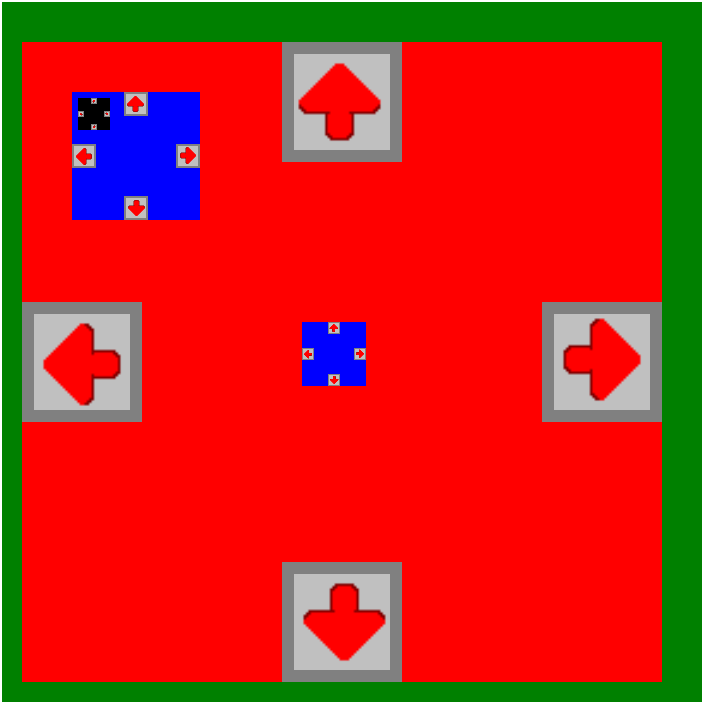
\includegraphics[width=0.4\textwidth]{GuiImg}\end{wrapfigure}
\noindent{\textit{Our Experiment:}} As shown in the figure, counting both \Q@SafeMovable@s and \Q@Button@s, our main method creates $21$ widgets: a top level (green) \Q@SafeMovable@ without buttons, containing $4$ (red, blue, and black) \Q@SafeMovable@s with
$4$ (gray) buttons each. When a button is pressed it moves the containing \Q@SafeMovable@ a small amount in the corresponding direction.
%Each container has 4 gray buttons one for each cardinal direction.
% In our set up
% the top level \Q@SafeMovable@
% contains a big red \Q@SafeMovable@
%  containing $2$ smaller blue \Q@SafeMovable@. One of those contains a tiny black \Q@SafeMovable@.
%Our invariant is that everything in every movable container (and the top level component) should 
%-be inside the container 
%-not overlap with anyhing else inside
%Our containers represent boxes that completley contain other non-overlapping boxes.
This set up is not overly involved, the maximum nesting level of \Q@Widget@s is $5$.
Our main method automatically presses each of the $16$ buttons once. In L42, using the approach of this paper, this resulted in $77$ calls to \Q@SafeMovable@'s invariant.

\textit{Comparison with visible state semantics:}
As an experiment we set our implementation to generate invariant checks following the approach for visible state semantics (the one used by Eiffel\footnote{We also tried the approach of D~\cite{Alexandrescu:2010:DPL:1875434,DRef} where invariants are instead checked on public method calls, but not private ones; however this produced identical results in our test case.
We expect all (sound) runtime approaches based on visible state semantics ~\cite{feldman2006jose,fahndrich2010embedded,abercrombie2002jcontractor,tran2003design}
to produce similar results.
}), where the invariant is instead checked at the start and end of \emph{every} unqualified method call%
\footnote{L42 follows the Eiffel uniform access principle: field accesses are the same as method calls.}
(i.e. on \Q@this@)
%though 42 represents field accesses as method calls, for a fair comparison with conventional OO approach, we do not treat field accesses on \Q@SafeMovable@s within the \Q@SafeMovable@ class itself as public method calls
% D and Eiffel have slightly different interpretation of
% visible state semantic when qualified/unqualified method calls or field accesses are performed.
% However, in our GUI example those corner cases are
% not relevant. To be sure, we implemented both of their strategies and obtained the same results.
of \Q@SafeMovable@, including the simple getters implementing the \Q@Widget@ interface. When we ran our test case following this approach, the invariant was called $52,734,053$ times (it took about $4$ days to run), in comparison to the $77$ we got when using our invariant protocol. The number of checks is exponential in the depth of the GUI: the invariant of a \Q@SafeMovable@ will call the \Q@width@, \Q@height@, \Q@left@, and \Q@top@ methods of its children, which may themselves be \Q@SafeMovable@s, and hence such calls will invoke further invariant checks. % Since we only use \Q@this@ to perform method calls, the invariant is not recursively checked on \Q@this@, if it were we would get an infinite recursion.
% Note that 42 represents field accesses as method calls, this is similar to the Eiffel uniform access principle; but for a fair comparison with D we treat private accesses to them like field accesses.


% It can be surprising to see such extreme difference. We ran our example with less widgets, and our results suggest an exponential growth in the cost of the conventional approach. For example by removing 2 containers (and their 8 buttons) we get....
% We now explain how this exponential explosion happens:
% For the outer-most box to check its invariant, it needs to call methods \Q@left,top,height@ and \Q@with@ to all its contained widgets.
% If one of those widget has \Q@invariant@, when such public method is called,
% its \Q@invariant@ is checked (twice). This requires to call \Q@left,top,height@ and \Q@with@ to all its contained widgets, some of those may also have \Q@invariant@s.

% In literature there is attention to prevent method called from an invariant to call public methods on \Q@this@; it would cause the system to go in loop.
% However when calling methods on other objects is allowed, if those objects have invariant, this cause the aforementioned explosion. 

% Our example also shows that the restrictions of TM's and OC's are flexible enough to encode interactive GUI programs, where widgets may circularly reference other widgets.
% In order to perform this case study, we had to first implemented a simple Gui Library in L42. This library uses object capabilities to draw the widgets on screen, as well as fetch and dispatch the events.
% The gui library abstract away all the details of drawing and events; the user code need only to provide concrete classes implementing the \Q@Widget@ interface.

\textit{Spec\# comparison:}
We also encoded our example in Spec\#\footnote{We compiled Spec\# using the latest available source (from 19/9/2014). The verifier available online at \url{rise4fun.com/SpecSharp} behalves differently.}, which like L42, statically verifies aliasing/ownership properties, as well as the admissibility of invariants.
% To keep the Spec\# code aligned with the L42 one, 
% we do not use a .NET GUI library, but we just simulate the behaviour of L42, without actually opening a window.
The backend of the L42 GUI library is written in Java, and we did not port it to Spec\# rather we just simulate the backend, and don't actually display a GUI in Spec\#.

We ran our code through the Spec\# verifier (powered by Boogie~\cite{DBLP:conf/fmco/BarnettCDJL05}), which only gave us $2$ warnings\footnote{We used \Q@assume@ statements, equivalent to Java's \Q@assert@, to dynamically check array bounds. %. and value presence.
This aligns the code with L42, which also performs such checks at runtime.}: that the invariant of \Q@SafeMovable@ was not known to hold at the end of its constructor and \Q@dispatch@ method; like our system however Spec\# checks this at runtime. As such the code is equivalently verified in both Spec\# and L42; in particular it performed exactly the same number ($77$) of runtime invariant checks.\footnote{
We also encoded our GUI in Microsoft Code Contracts~\cite{DBLP:conf/sac/FahndrichBL10}, whose unsound heuristic also run the invariant checking $77$ times; however Code Contract does not enforce the
encapsulation of \Q@children@, thus their approach would not be sound in our context.}

% Assuming that Spec\#'s verifier is sound, this means that our code is equally verified in Spec\# and L42, providing a reasonable comparison.
% Both Spec\# and L42 did the same thing:
% they statically verify ownership/aliasing annotations,
% they check the admissibility/valididty of a the invariant code and finally 
% they perform sufficient runtime-checking of the invariant.
% We used the Boogie static checker to verify all the aliasing/ownership properties needed to
% ensure that the $77$ run-time invariant checks soundly enforce that the invariant holds when is expected.
% This of course includes preventing the Gui to ever display two overlapping Widget. 

%\end{itemize}
%The result is the same of L42: the invariant is checked $77$ times, and in exactly the same locations of L42.

We found it quite difficult to encode the GUI in Spec\#, due to its unintuitive and rigid ownership discipline. In particular we needed to use many more annotations, which were both longer and had greater variety. In the following table we summarise the annotation burden,
for the \emph{program} that defines and displays \Q@SafeMovable@ and our GUI, as well as the \emph{library} which defines \Q@Button@s, \Q@Widget@, and event handling.\footnote{We only count constructs Spec\# adds over C\# as annotations, we also do not count annotations related to array bounds or null checks.}:
\begin{center}\saveSpace\saveSpace
\begin{tabular}{ c  c  c  c  c}
 & Spec\# & Spec\# & L42 & L42 \\ 
 & \!\!program\!\! & library & \!\!program\!\! & library \\
\hline
 
\!\!\!Total number of annotations 
 	& $40$ & $19$ & $19$ & $18$ \\ \hline
% Totals 	 $59$ $37
\!\!\!Tokens (except \Q@.,;(){}[]@ and whitespace)\!\!\!
%(ecluding \Q@;,@ characters, white-space, or parentheses/brackets.) 
	& $106$ & $34$ & $18$ & $18$  \\  \hline
% $140$  & $37$
Characters (with minimal whitespace) 
	& $619$ & $207$ & $74$ & $60$ \\ \hline
%  $826$ $134$
\end{tabular}
\end{center}

To encode the GUI example in L42, the only annotations we needed were the 3 type modifiers: \Q@mut@, \Q@read@, and \Q@capsule@.
% , for a total of 
% $19$ annotations (one token each, $74$ characters in total).
Our Spec\# code requires, among others, purity, immutability, ownership, method pre/post conditions and method modification annotations. In addition, it requires the use of 4 different ownership functions including explicit ownership assignments. In total we used 18 different kinds of annotations in Spec\#.
Together these annotations can get quite long, such as the following precondition on \Q@SafeMovable@'s constructor: \\
\begin{tabular}{r}
\Q@requires Owner.Same(Owner.ElementProxy(children), children);@
\end{tabular}

% methods and field attributes as well as requires, ensures and modifies clauses, and finally also %explicit ownership assignment statements.
% Spec\# annotation can be involved, as for example \Q@requires Owner.Same(Owner.ElementProxy(children), children);@}

% To estimate the annotation burden we count the number of tokens (excluding \Q@.;,@ and parenthesis).
% This gave us $113$ tokens, that is more then $5$ times the amount needed in L42.
% The total annotation character count is $830$; $10$ times more then L42.


% 40   106+17=113 619+211
%main 11 annotations, 28 + 11 tokens, 118+65 characters
%safemovable 29 annotations, 78+6 tokens, 501+146 characters

%19   34   207+44
% auxLib // 14 annotations, 25 tokens, 155+44 characters
%guiLib// 5 annoations, 9 tokens, 52 characters

% Moreover, in L42 we only use $3$ different kinds of annotations, while in Spec\# we use $15$ kinds of annotations.

The Spec\# code also required us to deviate from the style of code we showed in our simplified version: we could not write a usable \Q@children@ method in \Q@Widget@ that returns a list of children, instead we had to write \Q@children_count()@ and \Q@children(int i)@ methods; we also needed to create a trivial class with a \Q@[Pure]@ constructor (since \Q@Object@'s one is not marked as such). In contrast, the only strange thing we had to in L42 was creating \Q@Box@es by using 
an additional variable in a nested scope.
This is needed to delineate scopes for promotions.
Based on these results, we believe our system is significantly simpler and easier to use.
% On the basis of these results we believe  that our system is easier to use for programmers that are not experts in software verification.

\textit{The Box Pattern:}
Our design, using an inner \Q@Box@ object is a common pattern in static verification: where one encapsulates all relevant mutating state into an encapsulated sub object which is not exposed to users.

% We also found natural to use the box pattern also in Spec\# requires.
Both our L42 and Spec\# code required us to use the box pattern for our \Q@SafeMovable@, due to the circular object graph caused by the \Q@Action@s of \Q@Button@s needing to change their enclosing \Q@SafeMovable@ position.
% Also the implementation of the minimal GUI library (that our \Q@SaveMovable@ builds upon) has a much lower annotation burden.
%\LINE

\textit{The transform pattern:}
% A capsule mutator method is essentially a mutation of a field, which is guaranteed to not see the \Q@this@ object.
% Thus, if \Q@this@ is made invalid during  the method's execution, we could not observe it until after the method completes.
Suppose we want to scale a \Q@Widget@, we could add \Q@mut@ setters for \Q@width@, \Q@height@, \Q@left@, and \Q@top@ in the \Q@Widget@ interface. However, if we also wish to scale its children, we have a problem since \Q@Widget.children@ returns a \Q@read Widgets@, which does not allow mutation. We could of course add a \Q@mut@ method \Q@zoom@ to the \Q@Widget@ interface, however this does not scale if more operations are desired. If instead \Q@Widget.children@ returned a \Q@mut Widgets@, it would be difficult for \Q@Widget@ implementations, such as \Q@SafeMovable@, to keep control of their ROGs.

% In the above \Q@SafeMovable@ we only had one capsule mutator: \Q@dispatch@. However suppose a \Q@Widget@ wants to directly mutate it's descendents, however it can't do that since \Q@Widget.children@ returns a \Q@read Widgets@, if it returned a \Q@mut Widgets@ then \Q@SafeMovable@ could not be implement, as it's children are contained inside a capsule-field. 
% At first glance, it may seem that capsule mutators allow only very limited kinds %of mutation.
% This is however not the case. 

% Consider the following
% simple pattern to allow flexible use of encapsulated content: define a

A simple and practical solution would be to define a \Q@transform@ method in \Q@Widget@, and a \Q@Transformer@ interface 
like so:\footnote{A more general transformer could return a generic \Q@read R@.}
\saveSpace
\begin{lstlisting}
interface Transformer<T> {method Void apply(mut T elem);}
interface Widget {..
  mut method Void top(Int that);//setters for immutable data
  mut method read Void transform(Transformer<Widgets> t);
}//transformers for possibly encapsulated data
class SafeMovable {..
  mut method Void transform(Transformer<Widgets> t) {
    return t.apply(this.box.c);}} // Well typed capsule mutator
\end{lstlisting}\saveSpace
% Note that the code above does not access a capsule field but merely calls a method that does; thus  it is \emph{not} a capsule mutator method, so it is not constrained by the restrictions on them. Code like the above would also allow one to mutate multiple capsule fields in one method.
%Our pattern cooperates with the language’s restrictions to ensure each mutation is completed as a separate operation, that is perceived by the rest of the system %as if it was atomic.%
%,  i.e. they can't see or update the other capsule fields.
The \Q@transform@ method offers an expressive power similar to \Q@mut@ getters, but prevents \Q@Widgets@ from leaking out.  With a \Q@Transformer@, a \Q@zoom@ function could be simply:
\saveSpace\begin{lstlisting}
static method Void zoom(mut Widget w) {
  w.transform(ws -> {for(wi:ws){zoom(wi,scale);}});
  w.width(w.width()/2); ..; w.top(w.top()/2); }
\end{lstlisting}\saveSpace
\saveSpace
\saveSpace
% One of the advantages of this approach is that a the \@zoom@ method can be written by anyone anywhere

% \begin{lstlisting}[escapechar=\%]
%// Lambda Expression that creates a new Transformer<...>
%this.transform(l -> l.add(new MyWidget(..)))
%\end{lstlisting}
%//`i' is captured by the closure.
%// `imm' and `capsule' varaibles can be captured.

%    %\Comment{}%this.items.add(i);
%    // Cant instead capture `this': it can't be typed %as `imm'
%    // since `ItemTransformer.transform()' is an %`imm' method
%  })
%}
%  // instead of:
  %\Comment{}%this.exposeItems().add(i)

%Note that the code above does not access a capsule field but merely calls a method that does; thus
%it is \emph{not} a capsule mutator method, so it is not constrained by the restrictions on them. Code like the above would also allow one to mutate multiple capsule fields in one method.
%Our pattern cooperates with the language’s restrictions to ensure each mutation is completed as a separate operation, that is perceived by the rest of the system
%as if it was atomic.%
%,  i.e. they can't see or update the other capsule fields.

\begin{comment}
\subsection{Family, a worst case scenario for L42}
%\noindent\textit{Family, a worst case scenario for L42}
For our second case study, we wished to make an example where the performance of L42 and the conventional approach was similar. We forged an example when a \Q@Family@ has a list of parents and a list of children;
all the children need to be younger then their parents and every \Q@Person@ need to have a non empty name and a positive age.  
We model the pass of time with a \Q@processDay@ method, and we simulate $3$ years of life (that is, $3\times365$ days) of a family of $4$.
The age of a \Q@Person@ grow when its birthday is processed.
Notably, \Q@processDay@ is a \Q@mut@ method that can potentially mutate any person in the system, thus
L42 have to run a lot of invariant checks. The object graph here is very shallow: the \Q@Family@ holds the \Q@Person@s and that is it.
However, even in this case we get about $9$ times less invariant calls: $19403$ with visible state semantic  and $2210$ in L42.
%Also the \Q@Family@ example uses the box pattern.

\subsection{Expressiveness}
%\noindent\textit{Expressiveness:}
Finally, in our this third case study we 
shown that even if we do not aim to expressiveness, but to simplicity, soundness and efficiency, we are still able to express a reasonable amount of cases.
We encoded in L42 all the examples present in papers~\cite{??}.
We can express all the examples except ....
Again, we quantify the annotation burden and we discover....

%\subsection{The transform pattern}
\end{comment}

%\begin{lstlisting}[escapechar=\%]
%class List {
%  mut List prev;
%  mut List next;
%  Object elem;  
%  read method Bool ok() {
%    return this.next.prev==this && this.prev.next==this &&..;}
%  read method Int size(){
%    if(next==this){return 1;} return next.size()+1;}}
%\end{lstlisting}
%Clearly the \Q@mut@ fields of \Q@List@ cannot be marked as \Q@capsule@.
%However, only \Q@capsule@ and \Q@imm@
%fields can be accessed in \validate.
%Thus, \Q@.innerValidate()@ can not be the \Q@invariant@ method for \Q@List@.
%The solution is to use a `box' over our \Q@List@, and to validate our `box':
%
%\loseSpace\loseSpace\loseSpace
%\begin{lstlisting}[escapechar=\%]
%class ListBox { 
%  capsule List inner;
%  read method imm Bool invariant() {return this.inner.ok();}
%  read method Int size(){ return this.inner.size();}
%\end{lstlisting}
%\saveSpace
%Encoding this example in Spec\# would be much more verbose (see case study XX) and still require
%a \Q@ListBox@ object,
%while the visible state semantic of Eiffel or D would cause an large amount of \Q@invariant@ checks
%if the list had any recursive method; consider for example the \Q@size@ method:
%if there was an invariant with visible state semantic on \Q@List@, calling \Q@List.size()@ would require 
%calling \Q@List.invariant()@ before and after the method execution. If the list has more then one element, the recursive \Q@size@ call would also call the invariant twice.
%We would also want to create forwarding methods in \Q@ListBox@ for all public methods defined in \Q@List@. This approach allows the validation of many interesting and practically useful data-structures.
%However the limitations of capsule mutator methods mean that any \Q@mut@ methods in \Q@ListBox@ taking \Q@read@ or \Q@mut@ parameters, or returning \Q@mut@, cannot be trivially forwarded.
%% since they necessitate mutating a \Q@capsule@, instead complicated and involved forwarding would be needed, if it is even possible.
%Our example is about a list of immutable objects.
%To instead validate a list of \Q@mut@ objects we would need to use our box pattern not just around the list,
%but around a section of data encapsulating both the list and all the contained elements.
%This is because our simple \Q@capsule@ modifier requires the whole ROG to be encapsulated.
%Conceptually, it would be better for the list (of mutable objects) to be validated by its
%head, since the behaviour of the contained objects is transparent to the validation criteria. 
%Our limitation relates to full encapsulation and contrasts with flexible encapsulation as in 
%ownership~\cite{ClarkeEtAl98}. However, neither traditional flexible encapsulation/ownership, nor our language are capable of verifying that \Q@List.elem@ is not (indirectly) referenced within \Q@ListBox.validate()@.
%
